\documentclass[a4paper, 14pt]{extreport}
\usepackage[utf8]{inputenc}
\usepackage[english,russian]{babel}
\usepackage{amssymb,amsfonts,amsmath,mathtext,cite,enumerate,float}
\usepackage{pgfplots}
\usepackage{graphicx}
\usepackage[inkscapeformat=png]{svg}
\usepackage{tocloft}
\usepackage{listings}
\usepackage{caption}
\usepackage{tempora}
\usepackage{titlesec}
\usepackage{setspace}
\usepackage{geometry}
\usepackage{indentfirst}
\usepackage{pdfpages}
\usepackage{enumerate,letltxmacro}
\usepackage{threeparttable}
\usepackage{hyperref}
\usepackage{flafter}
\usepackage{enumitem}
\usepackage{multirow}
\usepackage{mathtools}
\usepackage{longtable}
\usepackage[figure,table]{totalcount}
\usepackage{lastpage}

\lstdefinestyle{lang}{
	language={c++},
	basicstyle=\footnotesize\ttfamily,
	frame=single,
	tabsize=4,	
	breaklines=true
}

\setlist{nosep}
\hypersetup{pdfborder=0 0 0}

\newcommand{\ssr}[1]{\begin{center}\LARGE\bfseries{#1}\end{center} \addcontentsline{toc}{chapter}{#1}  }

\makeatletter
\renewcommand\LARGE{\@setfontsize\LARGE{22pt}{20}}
\renewcommand\Large{\@setfontsize\Large{20pt}{20}}
\renewcommand\large{\@setfontsize\large{16pt}{20}}
\makeatother

\RequirePackage{titlesec}
\titleformat{\chapter}[block]{\hspace{\parindent}\large\bfseries}{\thechapter}{0.5em}{\large\bfseries\raggedright}
\titleformat{name=\chapter,numberless}[block]{\hspace{\parindent}}{}{0pt}{\large\bfseries\centering}
\titleformat{\section}[block]{\hspace{\parindent}\large\bfseries}{\thesection}{0.5em}{\large\bfseries\raggedright}
\titleformat{\subsection}[block]{\hspace{\parindent}\large\bfseries}{\thesubsection}{0.5em}{\large\bfseries\raggedright}
\titleformat{\subsubsection}[block]{\hspace{\parindent}\large\bfseries}{\thesubsection}{0.5em}{\large\bfseries\raggedright}
\titlespacing{\chapter}{12.5mm}{-22pt}{10pt}
\titlespacing{\section}{12.5mm}{10pt}{10pt}
\titlespacing{\subsection}{12.5mm}{10pt}{10pt}
\titlespacing{\subsubsection}{12.5mm}{10pt}{10pt}

\makeatletter
\renewcommand{\@biblabel}[1]{#1.}
\makeatother

\geometry{left=30mm}
\geometry{right=10mm}
\geometry{top=20mm}
\geometry{bottom=20mm}

\onehalfspacing

\renewcommand{\theenumi}{\arabic{enumi}}
\renewcommand{\labelenumi}{\arabic{enumi}\text{)}}
\renewcommand{\theenumii}{.\arabic{enumii}}
\renewcommand{\labelenumii}{\asbuk{enumii}\text{)}}
\renewcommand{\theenumiii}{.\arabic{enumiii}}
\renewcommand{\labelenumiii}{\arabic{enumi}.\arabic{enumii}.\arabic{enumiii}.}

\renewcommand{\cftchapleader}{\cftdotfill{\cftdotsep}}

\addto\captionsrussian{\renewcommand{\figurename}{Рисунок}}
\DeclareCaptionLabelSeparator{dash}{~---~}
\captionsetup{labelsep=dash}

\captionsetup[figure]{justification=centering,labelsep=dash}
\captionsetup[table]{labelsep=dash,justification=raggedright,singlelinecheck=off}
\captionsetup[lstlisting]{labelsep=dash,justification=raggedright,singlelinecheck=off}

\newcommand{\floor}[1]{\lfloor #1 \rfloor}

\pgfplotsset{width=0.85\linewidth, height=0.5\columnwidth}

\linespread{1.3}

\parindent=1.25cm

\def\labelitemi{---}
\setlist[itemize]{leftmargin=1.25cm, itemindent=0.65cm}
\setlist[enumerate]{leftmargin=1.25cm, itemindent=0.55cm}

\newcommand{\specialcell}[2][c]{\begin{tabular}[#1]{@{}c@{}}#2\end{tabular}}
\frenchspacing


\begin{document}

\setlength{\cftbeforetoctitleskip}{-4mm}

\setcounter{page}{3}
\renewcommand{\contentsname}{\makebox[\textwidth][c]{\largeСОДЕРЖАНИЕ}}
\tableofcontents

\clearpage\ssr{ОБОЗНАЧЕНИЯ И СОКРАЩЕНИЯ}

В представленной расчетно-пояснительной записке используются следующие сокращения и обозначения:
\begin{description}[leftmargin=0pt]
	\item \noindent ПО --- программное обеспечение.
	\item \noindent ООП --- объектно-ориентированное программирование.
	\item \noindent ЯП --- язык программирования.
\end{description}

\clearpage\ssr{ВВЕДЕНИЕ}

Компьютерная графика ---  это система методов, алгоритмов, программных и аппаратных средств для ввода, обработки и 
отображения графической информации, а также для преобразования данных в графическую форму.

Целью данной работы является разработка программного обеспечения для построения изображения  реалистичного
природного ландшафта.
Для достижения поставленной цели необходимо решить следующие задачи:
\begin{itemize}
	\item[---] провести анализ методов построения изображения карты высот;
	\item[---] провести анализ существующих алгоритмов построения изображения трехмерных объектов;
	\item[---] выбрать наиболее подходящие алгоритмы;
	\item[---] спроектировать архитектуру ПО;
	\item[---] выбрать средства реализации ПО;
	\item[---] реализовать ПО для построения изображения реалистичного природного ландшафта;
	\item[---] провести исследование зависимости количества объектов на сцене от временных характеристик программы.
\end{itemize}

\chapter{Аналитическая часть}

В этой части проводится анализ существующих алгоритмов генерации карты высот и построения изображений трехмерных 
объектов.

\section{Алгоритмы построения изображения карты высот}

Стохастический фрактал --- это фрактал, при построении которого случайным образом изменяются какие-либо параметры. 
Простым примером стохастического фрактала может служить траектория броуновского движения. На основе стохастических
фракталов и строятся карты высот~\cite{fractal}. Рассмотрим некоторые известные алгоритмы.

\subsection{Алгоритм diamond-square}

Алгоритм diamond-square начинает работу с двумерного массива размера $2^n + 1$. В четырёх угловых точках массива 
устанавливаются начальные значения высот. Шаги diamond и square выполняются поочередно до тех пор, пока все значения 
массива не будут установлены.~\cite{landscape}

\textbf{Шаг diamond.} Для каждого квадрата в массиве, устанавливается срединная точка, которой присваивается среднее
арифметическое из четырёх угловых точек плюс случайное значение.

\textbf{Шаг square.} Берутся средние точки граней тех же квадратов, в которые устанавливается среднее значение от четырёх 
соседних с ними по осям точек плюс случайное значение.

Пример шагов diamond и square представлен на рисунке~\ref{analytic:ds}.
\begin{figure}[h]
	\centering
	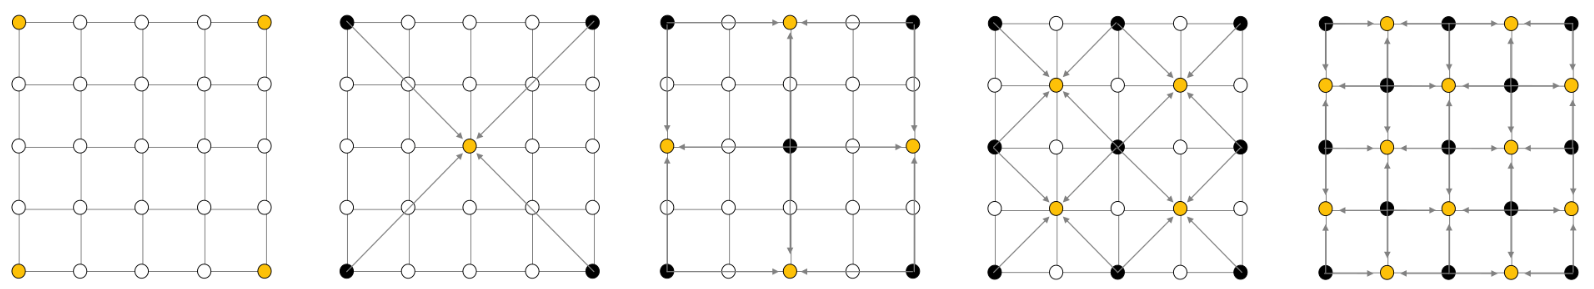
\includegraphics[scale=0.5]{tools/diamond-square.png}
	\caption{Шаги diamond и square в алгоритме diamond-square}
	\label{analytic:ds}
\end{figure}

\subsection{Шум Перлинга}

Шум Перлина --- это градиентный шум, состоящий из набора псевдослучайных единичных векторов (направлений градиента), 
расположенных в определенных точках пространства и интерполированных функцией сглаживания между этими точками. 
Реализация обычно включает три этапа: определение сетки случайных векторов градиента (рисунок~\ref{analytic:p1}), 
вычисление скалярного произведения векторов градиента и их смещений (рисунок~\ref{analytic:p2}) и интерполяция между 
этими значениями (рисунок~\ref{analytic:p3}). Алгоритм шума Перлина можно масштабировать в одномерном, двухмерном и 
трёхмерном виде. Более того, в алгоритм можно ввести четвертое временное измерение, позволяя алгоритму динамически 
изменять текстуры во времени.~\cite{landscape}

\begin{figure}[h]
	\centering
	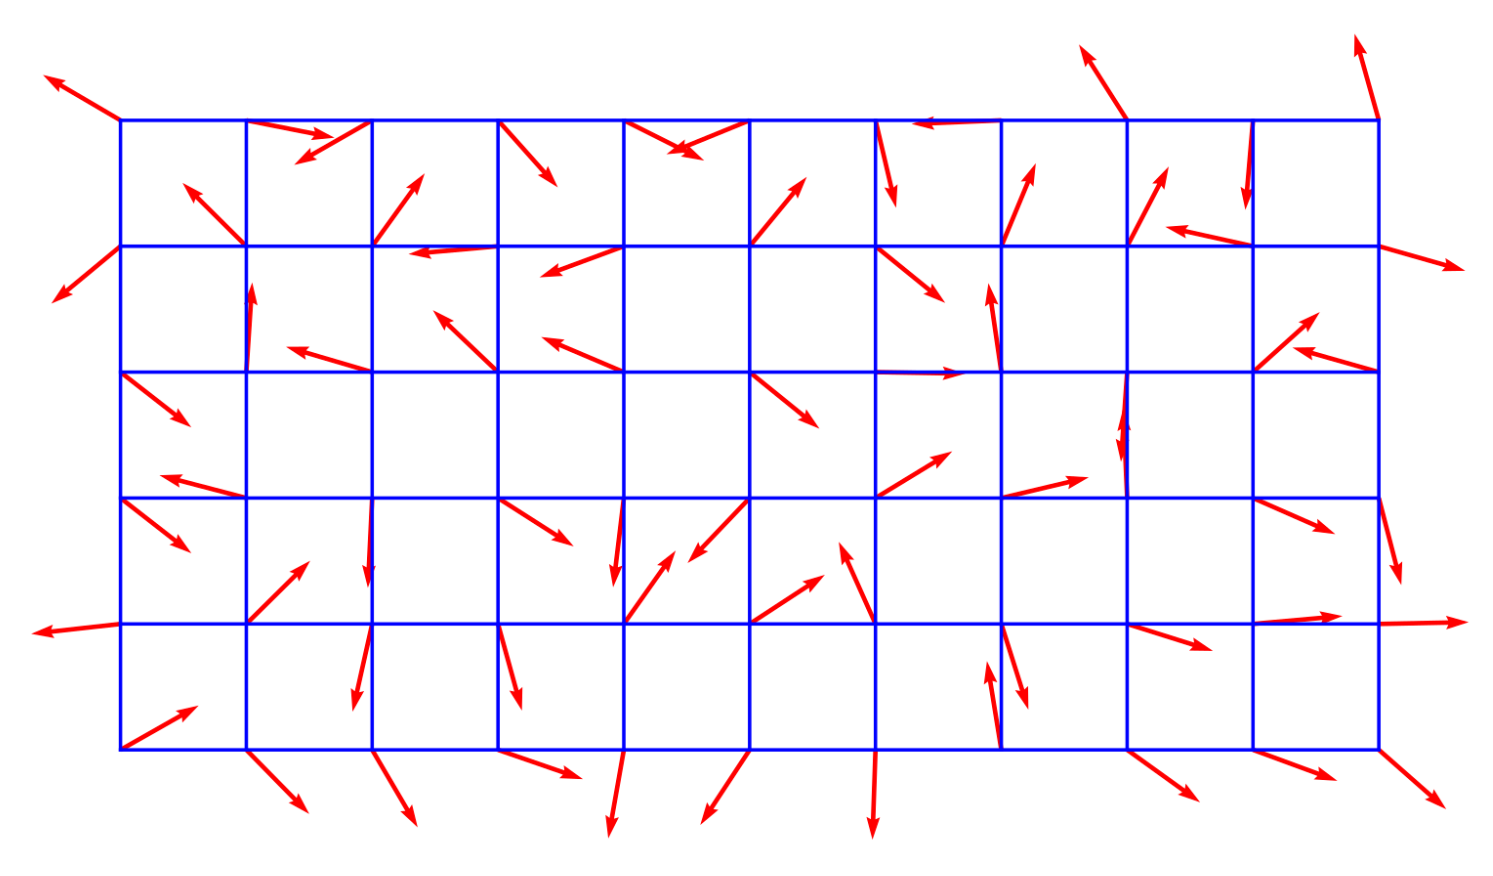
\includegraphics[scale=0.4]{tools/perling_1.png}
	\caption{Определение сетки случайных векторов}
	\label{analytic:p1}
\end{figure}

\begin{figure}[h]
	\centering
	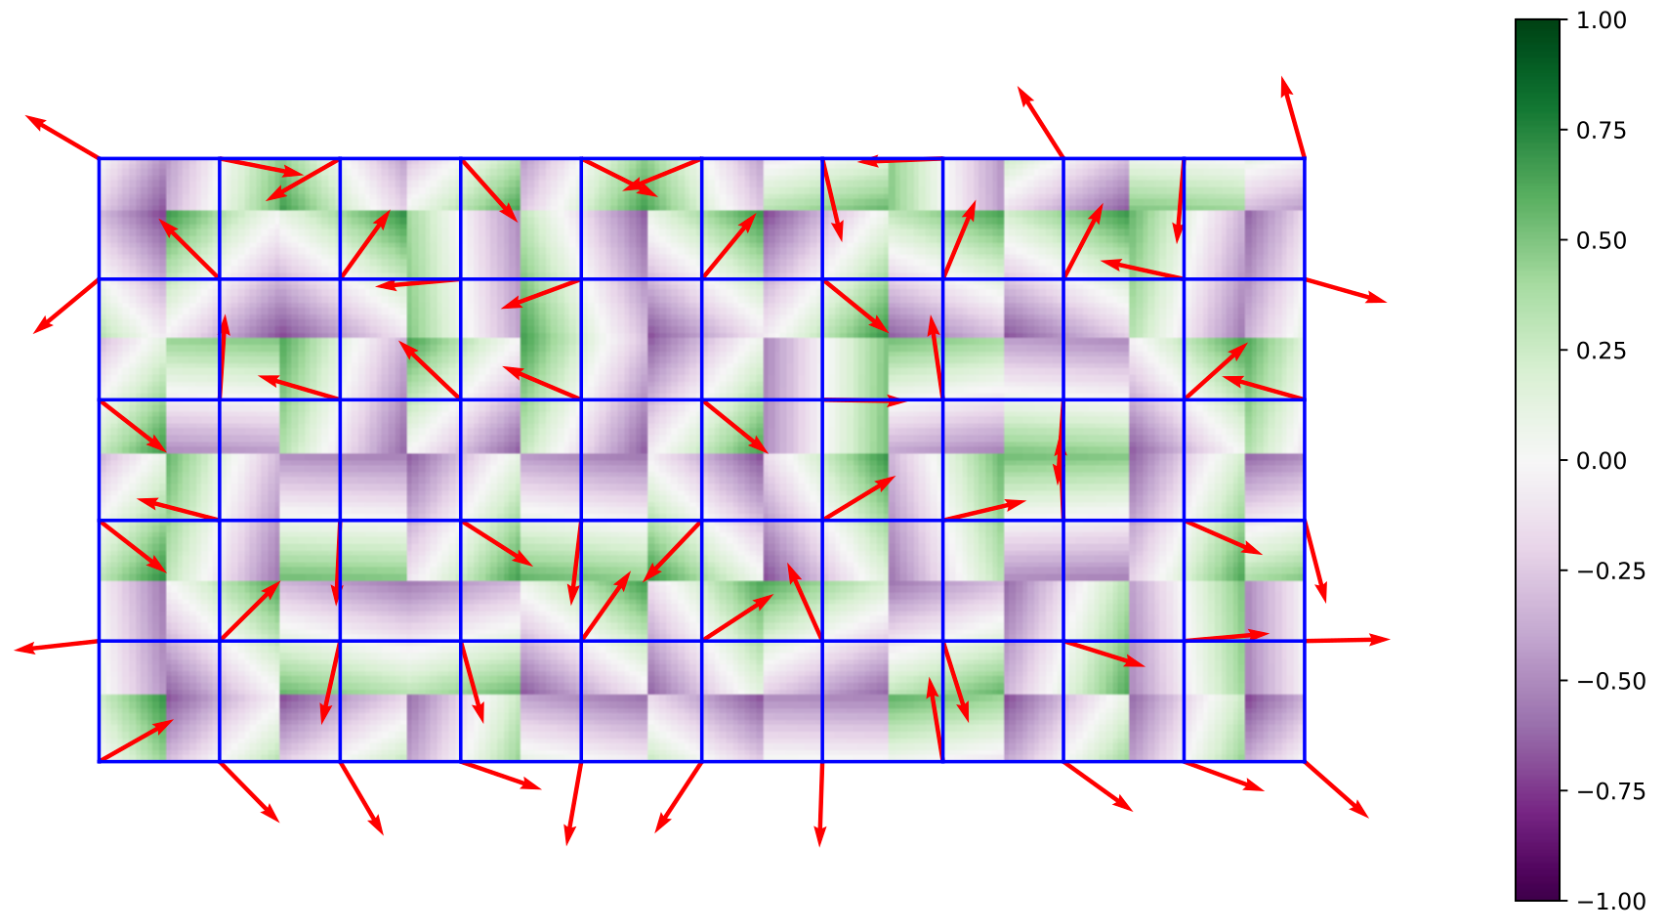
\includegraphics[scale=0.4]{tools/perling_2.png}
	\caption{Вычисление скалярного произведения вектора градиента и вектора смещения}
	\label{analytic:p2}
\end{figure}

\begin{figure}[h]
	\centering
	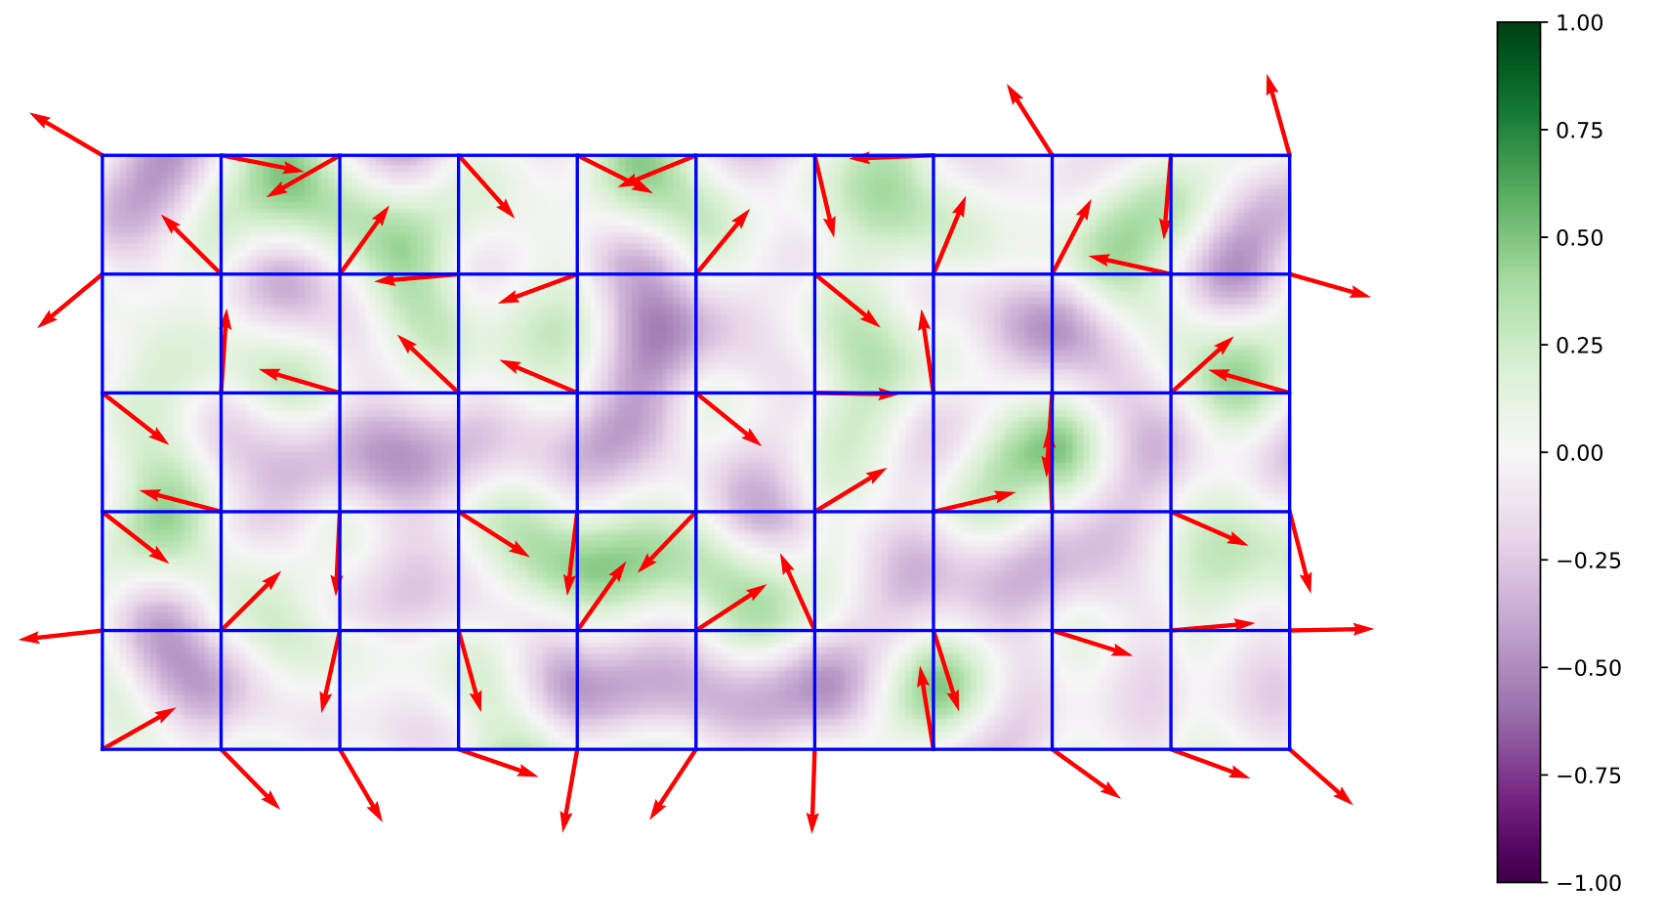
\includegraphics[scale=0.4]{tools/perling_3.png}
	\caption{Интерполяция между найденными значениями}
	\label{analytic:p3}
\end{figure}

\clearpage\section{Алгоритмы удаления невидимых линий и поверхностей}

Основной задачей при построения изображения трехмерного объекта является удаления невидимых объектов или частей
объектов. Невидимыми считаются те объекты или части объектов, которые перекрываются другими объектами. Выделяется
две группы алгоритмов решающих поставленную задачу~\cite{rodjers}:
\begin{itemize}
	\item Алгоритмы, работающие в объектном пространстве. Данные алгоритмы имеют привязку к мировой или физической 
	системе координат~\cite{rodjers}.
	\item Алгоритмы, работающие в пространстве изображения. Данные алгоритмы предполагают привязку к системе 	
	координат экрана или картинной плоскости, на которую производится проецирование изображаемых 
	объектов~\cite{rodjers}.
\end{itemize}

\subsection{Алгоритм Робертса}

Алгоритм работает в объектном пространстве, решая задачу только с выпуклыми телами. Выполняется в 3 этапа~\cite{rodjers}. 

\textbf{Первый этап} --- подготовка исходной матрицы $V$, которая задает информацию о каждой фигуре. 
Размерность матрицы --- $4 * n$, где $n$ -- количество граней тела. Каждый столбец матрицы представляет собой четыре 
коэффициента уравнения плоскости $ax + by + cz + d = 0$, проходящей через очередную грань.
Таким образом, матрица тела будет представлена в следующем виде:
\begin{equation}
	V = \begin{pmatrix}
		a_{1} & a_{2} & \ldots & a_{n}\\
		b_{1} & b_{2} & \ldots & b_{n}\\
		c_{1} & c_{2} & \ldots & c_{n}\\
		d_{1} & d_{2} & \ldots & d_{n}
	\end{pmatrix}
\end{equation}
Матрица тела должна быть сформирована корректно, то есть любая точка, расположенная внутри тела, должна располагаться 
по положительную сторону от каждой грани тела. В случае, если для очередной грани условие не выполняется, 
соответствующий столбец матрицы надо умножить на $-1$.  Для проведения проверки следует взять точку, расположенную 
внутри тела. Координаты такой точки можно получить путем усреднения координат всех вершин тела.

\textbf{Второй этап} --- удаления ребер, экранируемых самим телом, где рассматривается вектор взгляда $E = \{0, 0, -1, 0\}$.
Для определения невидимых граней достаточно умножить вектор $E$ на матрицу тела $V$. Отрицательные компоненты 
полученного вектора будут соответствовать невидимым граням.

\textbf{Третий этап} --- удаление невидимых ребер, экранируемых другими телами сцены. 
Для определения невидимых точек ребра требуется построить луч, соединяющий точку наблюдения с точкой на ребре. 
Точка будет невидимой, если луч на своем пути встречает в качестве преграды рассматриваемое тело. 
Если тело является преградой, то луч должен пройти через тело.  Если луч проходит через тело, то он находится по 
положительную сторону от каждой грани тела.

В данном алгоритме главным недостатком является его вычислительная трудоемкость равная $O(n^2)$, где $n$ --- количество 
объектов на сцене~\cite{rodjers}. Также все тела на сцене должны быть выпуклыми, что приводит к дополнительным проверкам.
Однако, работа в объектном пространстве и высокая сложность вычислений обеспечивает высокую точность результата.

\subsection{Алгоритм прямой трассировки лучей}

В методе прямой трассировки предполагает построения траекторий лучей от всех источников света ко всем точкам всех 
объектов сцены, отражаются и преломляются или проходят сквозь него и в результате достигает наблюдателя. Такие лучи 
называются первичными. Если объект не является отражающим или прозрачным, то траектория луча на этой точке 
обрывается~\cite{ulianov}.

Основным недостатком алгоритма является излишне большое число рассматриваемых лучей, приводящее к существенным 
затратам вычислительных мощностей, так как лишь малая часть лучей достигает точки наблюдения~\cite{livshic}.

\subsection{Алгоритм обратной трассировки лучей}

Отслеживать пути лучей от источника к наблюдателю неэффективно с точки зрения вычислений, поэтому наилучшим способом 
будет отслеживание путей в обратном направлении, то есть от наблюдателя к объекту. Лучи испускаются из камеры, 
пронизывая каждый пиксель сцены. После этого определяют пересечение первичного луча с объектами сцены. 
Если оно было установлено, вычисляют интенсивность пикселя, учитывая положения источников света~\cite{eromin}.
Считается, что наблюдатель расположен на положительной полуоси $z$ в бесконечности, поэтому все световые лучи 
параллельны оси $z$. В ходе работы испускаются лучи от наблюдателя и ищутся пересечения луча и всех объектов сцены. 
В результате пересечение с максимальным значением $z$ является видимой частью поверхности и атрибуты данного объекта 
используются для определения характеристик пикселя, через центр которого проходит данный световой луч.
Для расчета эффектов освещения сцены проводятся вторичные лучи от точек пересечения ко всем источникам света. Если на 
пути этих лучей встречается непрозрачное тело, значит, данная точка находится в тени~\cite{rodjers}.

Несмотря на более высокую эффективность алгоритма в сравнении с прямой трассировкой лучей, данный алгоритм считается 
достаточно медленным, так как в нем происходит точный расчет сложных аналитических выражений для нахождения 
пересечения с рассматриваемыми объектами~\cite{eromin}.

\subsection{Алгоритм Варнока}

Алгоритм Варнока работает в пространстве изображения и позволяет определить, какие грани или части граней объектов сцены 
видимы, а какие заслонены другими объектами~\cite{porev}. Алгоритм прелагает разбиение области изображения на более 
мелкие окна, и для каждого такого окна определяются связанные с ней многоугольники и те, видимость которых можно 
определить, изображаются на сцене.

В качестве граней обычно выступают выпуклые многоугольники, алгоритмы работы с ними эффективнее, чем с произвольными 
многоугольниками. Окно, в котором необходимо отобразить сцену, должно быть прямоугольным. Алгоритм работает 
рекурсивно, что является его главным недостатком, на каждом шаге анализируется видимость граней и, если  нельзя <<легко>> 
определить видимость, окно делится на 4 части и анализ повторяется отдельно для каждой из частей. 

\subsection{Алгоритм, использующий Z-буфер}

Алгоритм, использующий z-буфер, является одним из самых простых и широко используемых и работает в пространстве 
изображения. Идея z-буфер является простым обобщением идеи о буфере кадра~\cite{rodjers}. Используется два буфера:
\begin{itemize}
	\item[---] буфер кадра, который используется для запоминания атрибутов (интенсивности) каждого пикселя;
	\item[---] z-буфер --- отдельный буфер глубины, используемый для запоминания координаты z каждого пикселя.
\end{itemize}

Первоначально в z-буфере находятся минимально возможные значения z, а в буфере кадра располагаются пиксели, 
описывающие цвет фона. В процессе работы глубина z каждого нового пиксела, который нужно занести в буфер кадра, 
сравнивается с глубиной того пикселя, который уже занесен в z-буфер. Если новый пиксель расположен ближе к наблюдателю, 
чем предыдущий, то он заносится в буфер кадра и происходит корректировка z-буфера. В противном случае никаких действий 
не производится~\cite{gonhchan}.

Основным преимуществом алгоритма является то, что трудоемкость алгоритма увеличивается линейно в зависимости от 
количества объектов на сцене. Также нет необходимости в сортировке объектов~\cite{polsky}.

Основным недостатком является то, что алгоритм требователен к памяти из-за необходимости хранить два буфера.
Реализация эффектов прозрачности и устранения лестничного эффекта осложнена~\cite{polsky}.

\section{Выбор алгоритмов}

Для построения карты высот был выбран алгоритм diamond-square, так как его трудоемкость квадратично зависит от
размеров карты~\cite{fractal}.

В реализации программного обеспечения необходимо обеспечить возможность быстрого и плавного перемещения камеры, 
поэтому алгоритм должен иметь минимальную зависимость трудоемкости от количества объектов на сцене. Так как 
ограничений по объему памяти нет, то наиболее подходящим алгоритмом является алгоритм с использованием Z-буфера.

\section{Вывод}

В этом разделе были рассмотрены алгоритмы построения изображения карты высот и построения изображения трехмерных
объектов. Также были обоснованно выбраны алгоритмы для дальнейшего проектирования архитектуры ПО.

\chapter{Конструкторская часть}

В этой части представлены требования к ПО, а также описания алгоритмов.

\section{Требования к программному обеспечению}

Программа должна предоставлять пользователю следующие возможности:
\begin{itemize}
	\item[---] генерация случайной карты высот;
	\item[---] чтение карты высот из файла;
	\item[---] сохранение карты высот в файл;
	\item[---] построение ландшафта по карте высот;
	\item[---] задание положения источника света;
	\item[---] перемещение камеры.
\end{itemize}

\section{Описание алгоритма diamond-square}

На вход алгоритму подается два числа N и M --- высота и ширина карты высот. На выходе ожидается  --- матрица 
высот размером $N \times M$. 

На рисунках~\ref{constr:ds}--\ref{constr:build} представлена схема алгоритма diamond-square и рекурсивной функции $build$.

\begin{figure}[h]
	\centering
	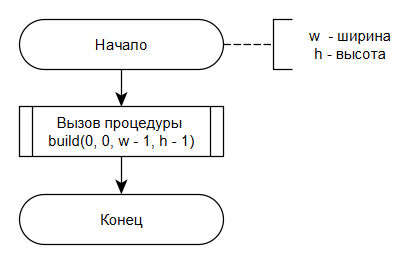
\includegraphics[scale=0.9]{tools/alg_ds.png}
	\caption{Схема алгоритма diamond-square}
	\label{constr:ds}
\end{figure}

\begin{figure}[h]
	\centering
	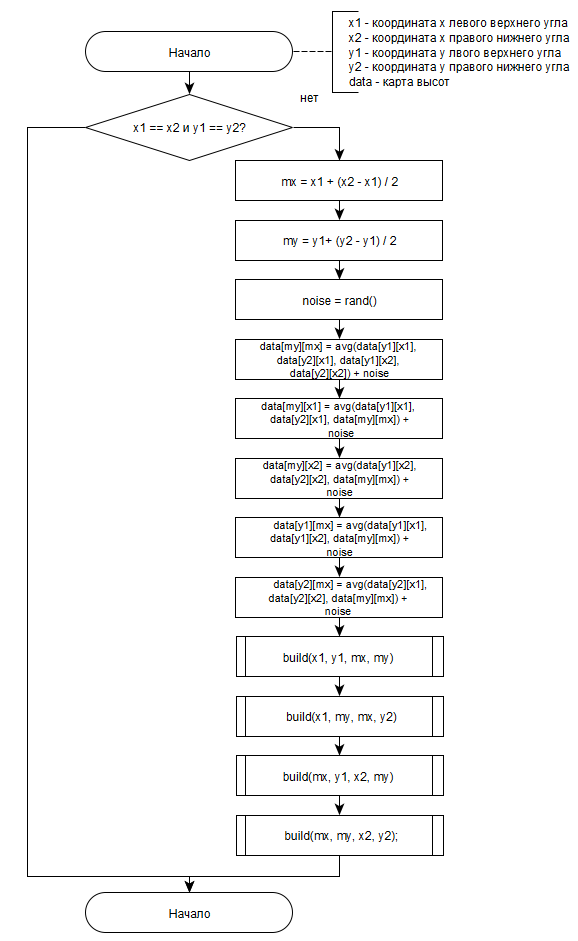
\includegraphics[scale=1.1]{tools/alg_build.png}
	\caption{Схема рекурсивной функции build}
	\label{constr:build}
\end{figure}

\clearpage\section{Схема алгоритма с использованием Z-буфера}

На вход алгоритму подается полигон, который необходимо отрисовать. На выходе --- буфер кадра.

На рисунке~\ref{constr:z} представлена схема алгоритма с использование Z-буфера.

\begin{figure}[h]
	\centering
	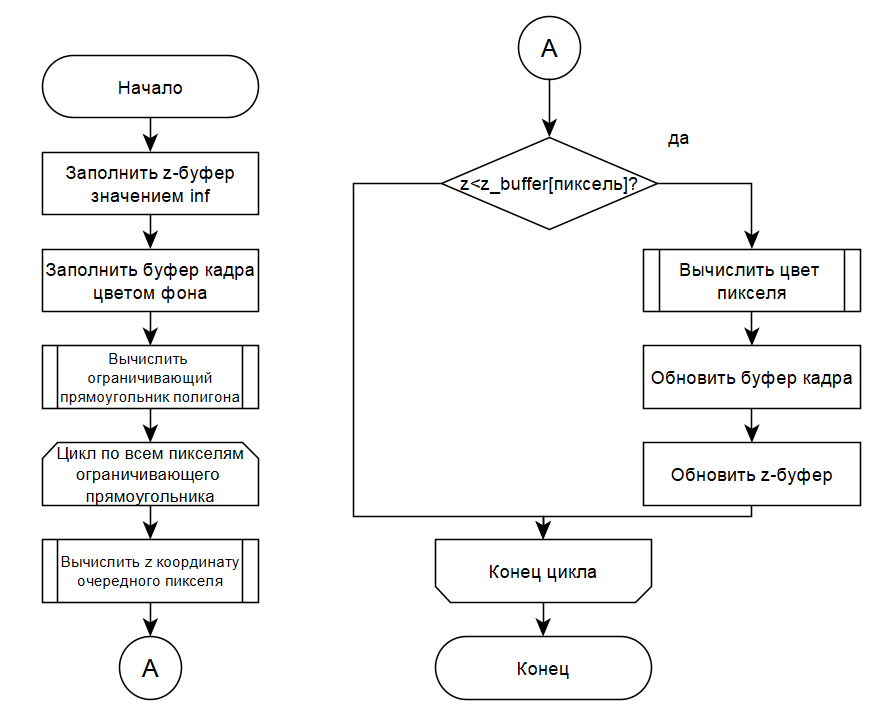
\includegraphics[scale=0.8]{tools/alg_z.png}
	\caption{Схема алгоритма с использованием Z-буфера}
	\label{constr:z}
\end{figure}

\section{Вывод}

В этой части было спроектировано программное обеспечение: описаны требования и представлены схемы базовых 
алгоритмов.

\chapter{Технологическая часть}

В этой части обоснован выбор средств реализации программного обеспечения, а также представлены коды написанных
алгоритмов.

\section{Средства реализации}

Для реализации алгоритмов был выбран язык C++~\cite{c++}. Выбор обусловлен следующим образом:
\begin{itemize}
	\item[---] язык поддерживает ООП парадигму;
	\item[---] в языке присутствует поддержка всех структур данных, выбранным по результатам проектирования;
	\item[---] средствами языка можно реализовать все алгоритмы, выбранные в результате проектирования;
	\item[---] поддерживает графические библиотеки, например, Qt~\cite{qt}.
\end{itemize}

\section{Реализация алгоритма diamond-square}

В листинге~\ref{lst:ds} приведено описание алгоритма diamond-square.
\begin{lstlisting}[style=lang, label=lst:ds,caption=Реализация алгоритма diamond-square]
void build(int x1, int y1, int x2, int y2)
{
    if (x2 - x1 <= 1 && y2 - y1 <= 1) return ;
    int mx = x1 + (x2 - x1) / 2, my = y1 + (y2 - y1) / 2;
    int noise = getRandValue() * (log2(x2 - x1) / log2(_width) * _alpha);
    if (_data[my][mx] == MAX_DEPTH - 1) {
        _data[my][mx] = getMiddleVal({_data[y1][x1], _data[y2][x1], _data[y1][x2], _data[y2][x2]});
        _data[my][mx] = fixValue(_data[my][mx] + noise);
    }
    if (_data[my][x1] == MAX_DEPTH - 1) {
        _data[my][x1] = getMiddleVal({_data[y1][x1], _data[y2][x1], _data[my][mx]});
        _data[my][x1] = fixValue(_data[my][x1] + noise);
    }
    if (_data[my][x2] == MAX_DEPTH - 1) {
        _data[my][x2] = getMiddleVal({_data[y1][x2], _data[y2][x2], _data[my][mx]});
        _data[my][x2] = fixValue(_data[my][x2] + noise);
    }
    if (_data[y1][mx] == MAX_DEPTH - 1) {
        _data[y1][mx] = getMiddleVal({_data[y1][x1], _data[y1][x2], _data[my][mx]});
        _data[y1][mx] = fixValue(_data[y1][mx] + noise);
    }
    if (_data[y2][mx] == MAX_DEPTH - 1) {
        _data[y2][mx] = getMiddleVal({_data[y2][x1], _data[y2][x2], _data[my][mx]});
        _data[y2][mx] = fixValue(_data[y2][mx] + noise);
    }

    build(x1, y1, mx, my);
    build(x1, my, mx, y2);
    build(mx, y1, x2, my);
    build(mx, my, x2, y2);
}

int main() {
    _data[0][0] = _rand.bounded(MAX_DEPTH, MAX_HEIGHT);
    _data[0][_width - 1] = _rand.bounded(MAX_DEPTH, MAX_HEIGHT);
    _data[_height - 1][0] = _rand.bounded(MAX_DEPTH, MAX_HEIGHT);
    _data[_height - 1][_width - 1] = _rand.bounded(MAX_DEPTH, MAX_HEIGHT);
    build(0, 0, _width - 1, _height - 1);
}
\end{lstlisting}

\section{Реализация алгоритма с использованием Z-буфера}

В листинге~\ref{lst:z} приведено описание алгоритма с использованием Z-буфера.

\begin{lstlisting}[style=lang, label=lst:z,caption=Реализация алгоритма с использованием Z-буфера]
void Render::renderTriangle(QVector<QPointF> &projs, QVector<QVector3D> &points, QVector<QVector3D> &normals, QVector<int> &face,
                            QColor &color, Light &light) {
    QPointF p0 = projs[face[0]], p1 = projs[face[1]], p2 = projs[face[2]];
    QVector3D n0 = normals[face[0]], n1 = normals[face[1]], n2 = normals[face[2]];
    double z0 = points[face[0]].z(), z1 = points[face[1]].z(), z2 = points[face[2]].z();
    QVector3D v0 = points[face[0]], v1 = points[face[1]], v2 = points[face[2]];

    if ((p1.y() - p2.y()) * (p0.x() - p2.x()) + (p2.x() - p1.x()) * (p0.y() - p2.y()) < 1e-6) return;

    int minX = std::max(0, static_cast<int>(std::floor(std::min({p0.x(), p1.x(), p2.x()}))));
    int maxX = std::min(_width - 1, static_cast<int>(std::ceil(std::max({p0.x(), p1.x(), p2.x()}))));
    int minY = std::max(0, static_cast<int>(std::floor(std::min({p0.y(), p1.y(), p2.y()}))));
    int maxY = std::min(_height - 1, static_cast<int>(std::ceil(std::max({p0.y(), p1.y(), p2.y()}))));

    for (int y = minY; y <= maxY; ++y) {
        for (int x = minX; x <= maxX; ++x) {
            QPointF point(x + 0.5, y + 0.5);

            QVector3D baric = calcBaric(point, p0, p1, p2);
            if (baric.x() < 0 || baric.y() < 0 || baric.z() < 0) continue;

            double z = baric.x() * z0 + baric.y() * z1 + baric.z() * z2;

            QVector3D normal = calcNormals(n0, n1, n2, baric.x(), baric.y(), baric.z());
            QVector3D worldPoint = baric.x() * v0 + baric.y() * v1 + baric.z() * v2;
            QColor pix_color = calcShadow(normal, light, worldPoint, color);

            if (z < _z_buffer[y][x]) {
                _z_buffer[y][x] = z;
                _image_buffer[y][x] = pix_color;
            }
        }
    }
}

QColor Render::calcShadow(QVector3D &normal, Light &light, QVector3D &point, QColor &baseColor) {
    QVector3D lightDir = (light.getPos() - point);
    lightDir.normalize();
    double intensity = QVector3D::dotProduct(lightDir, normal);
    if (intensity > 0)
        return QColor(baseColor.red()*intensity, baseColor.green()*intensity, baseColor.blue()*intensity);
    return Qt::black;
}

QVector3D Render::calcNormals(QVector3D n0, QVector3D n1, QVector3D n2, double alpha, double beta, double gamma) {
    QVector3D result;
    result.setX(n0.x() * alpha + n1.x() * beta + n2.x() * gamma);
    result.setY(n0.y() * alpha + n1.y() * beta + n2.y() * gamma);
    result.setZ(n0.z() * alpha + n1.z() * beta + n2.z() * gamma);

    return result;
}

QVector3D Render::calcBaric(QPointF &point, QPointF &p0, QPointF &p1, QPointF &p2) {
    double denom = (p1.y() - p2.y()) * (p0.x() - p2.x()) + (p2.x() - p1.x()) * (p0.y() - p2.y());
    double alpha = ((p1.y() - p2.y()) * (point.x() - p2.x()) + (p2.x() - p1.x()) * (point.y() - p2.y())) / denom;
    double beta = ((p2.y() - p0.y()) * (point.x() - p2.x()) + (p0.x() - p2.x()) * (point.y() - p2.y())) / denom;
    double gamma = 1.0 - alpha - beta;
    return QVector3D(alpha, beta, gamma);
}
\end{lstlisting}

\section{Вывод}

В этой части были приведены средства реализации ПО. Также было реализовано программное обеспечение, выполняющее
построение изображения реалистичного природного ландшафта.

\chapter{Исследовательская часть}

\clearpage\ssr{ЗАКЛЮЧЕНИЕ}

Цель данной работы была достигнута: разработано программное обеспечение для построения изображения  реалистичного
природного ландшафта. Были решены все задачи:
\begin{itemize}
	\item[---] проведен анализ методов построения изображения карты высот;
	\item[---] проведен анализ существующих алгоритмов построения изображения трехмерных объектов;
	\item[---] выбраны наиболее подходящие алгоритмы;
	\item[---] спроектирована архитектура ПО;
	\item[---] выбраны и обоснованы средства реализации ПО;
	\item[---] реализовано ПО для построения изображения реалистичного природного ландшафта;
	\item[---] проведено исследование зависимости количества объектов на сцене от временных характеристик программы.
\end{itemize}

\addcontentsline{toc}{chapter}{СПИСОК ИСПОЛЬЗОВАННЫХ ИСТОЧНИКОВ}
\renewcommand{\bibname}{СПИСОК ИСПОЛЬЗОВАННЫХ ИСТОЧНИКОВ}
\begin{thebibliography}{}
	\bibitem{rodjers}  Дэвид Роджерс. Алгоритмические основы машинной графики --- М.: Мир, 1989, 512 с. (дата обращения: 
	09.09.2024)
	\bibitem{porev} Виктор Порев. Компьютерная графика --- СПб.: БХВ-Петербург, 2002, 432 с. (дата обращения: 
	09.09.2024)
	\bibitem{fractal} Д.И. Иудин, Е.В. Копосов. Фракталы: от простого к сложному --- Город: Нижний Новогород, ННГАСУ, 2012, 
	185 с. (дата обращения: 09.09.2024)
	\bibitem{landscape} Некоторые вопросы генерации реалистичных ландшафтов / [Электронный ресурс] // Режим доступа: 
	\url{https://scilead.ru/article/2213-nekotorie-voprosi-generatsii-realistichnikh-l} (дата обращения: 09.09.2024)
	\bibitem{livshic} Алгоритмические основы компьютерной графики / [Электронный ресурс] // Режим доступа: \url{https://
	libeldoc.bsuir.by/bitstream/123456789/2530/2/Livshic_al.pdf}  (дата обращения: 09.09.2024)
	\bibitem{polsky} Компьютерная графика / [Электронный ресурс] // Режим доступа: \url{https://mf.bmstu.ru/info/faculty/kf/caf/	
	k3/subjects/Computer_graphics/materials/CG_RGR.pdf} (дата обращения: 09.09.2024)
	\bibitem{gonhchan} Алгоритм удаления невидимых поверхностей на основе программных проверок видимости / 
	[Электронный ресурс] // Режим доступа: \url{https://www.ispras.ru/proceedings/docs/2018/30/2/isp_30_2018_2_81.pdf}  (дата 
	обращения: 09.09.2024)
	\bibitem{ulianov} Метод трассировки лучей как основная технология фотореалистичного рендеринга / [Электронный 
	ресурс] // Режим доступа: \url{https://fundamental-research.ru/ru/article/view?id=39706} (дата обращения: 09.09.2024)
	\bibitem{eromin} Трассировка лучей на распределенной вычислительной системе / [Электронный ресурс] // Режим доступа: 
	\url{https://top-technologies.ru/article/view?id=38782} (дата обращения: 09.09.2024)
	\bibitem{light} Простые модели освещения / [Электронный ресурс] // Режим доступа: \url{https://grafika.me/node/344} (дата 	
	обращения: 09.09.2024)
	\bibitem{qt} All Qt Documentation / [Электронный ресурс] // Режим доступа: \url{https://doc.qt.io/all-topics.html} (дата 	
	обращения: 09.09.2024)
	\bibitem{c++} Документация по языку C++ / [Электронный ресурс] // Режим доступа: \url{https://learn.microsoft.com/ru-ru/
	cpp/cpp/?view=msvc-160} (дата обращения: 09.09.2024)
\end{thebibliography}

\clearpage\ssr{ПРИЛОЖЕНИЕ А}

\end{document}